%main.tex
\documentclass[a4paper]{article}
%其余为默认值,需要的话再添加控制参数,详见《入门手册》

%——————————————————————导言区——————————————————————

\usepackage{float}
\usepackage{color}

%——————————————————————设置页眉页脚——————————————————————
\usepackage{fancyhdr}
%\usepackage{lastpage}%获得总页数

%——————————————————————设置摘要——————————————————————
\renewcommand{\abstractname}{摘要}

%——————————————————————设置目录样式——————————————————————
\usepackage{titlesec}  
\usepackage{titletoc}
\usepackage{xfrac}
\contentsmargin{0pt}\renewcommand\contentspage{\thecontentspage}
\renewcommand\contentsname{\centerline{目\hspace{1em}录}}%目录 二字居中
\dottedcontents{section}[0.66cm]{\addvspace{5pt}}{1em}{6pt}
%\dottedcontents{section}[0.66cm]{\addvspace{5pt}}{1em}{5pt}
\dottedcontents{subsection}[1.40cm]{}{1.7em}{5pt}
\dottedcontents{subsubsection}[2.51cm]{}{2.4em}{5pt}
%更改目录样式,addvspace更改了sec之间的行间距

%——————————————————————设置中文字体——————————————————————
\usepackage{xeCJK}
%\usepackage[no-config,quiet]{fontspec}%使用电脑自带字体
\setCJKmainfont[BoldFont ={SimHei},ItalicFont ={SimSun}]{SimSun}%设置中文正体字体,BoldFont设置粗体和斜体样式对应的字体
\setCJKsansfont{SimHei}%设置无衬线样式对应字体
\setCJKmonofont{SimSun}%设置有衬线样式对应字体
\punctstyle{hangmobanjiao} %行末半角式:所有标点占一个汉字宽度,行首行末对齐
\setCJKfamilyfont{hei}{SimHei}                        
\newcommand{\hei}{\CJKfamily{hei}} 
\newcommand{\con}{Consolas}

%——————————————————————设置字号——————————————————————
\newcommand{\xiaoerhao}{\fontsize{18pt}{\baselineskip}\selectfont}
\newcommand{\sihao}{\fontsize{14pt}{\baselineskip}\selectfont}
\newcommand{\wuhao}{\fontsize{10.5pt}{\baselineskip}\selectfont}
\newcommand{\xiaowuhao}{\fontsize{9pt}{\baselineskip}\selectfont}

%——————————————————————设置间距——————————————————————
\usepackage{setspace}%使用间距宏包
\setlength{\parskip}{0.2\baselineskip}%段间距 这个一般是0.5
%\renewcommand{\baselinestretch}{1}%行间距

%——————————————————————设置数学字体——————————————————————
%\usepackage{mathpazo,pxfonts}%配合数学字体palatino linotype使用的
\usepackage{times,amsmath,txfonts}%配合数学字体times new roman使用的
\usepackage{bm}
\let\iint\relax\let\iiint\relax\let\iiiint\relax\let\idotsint\relax\usepackage{amsmath}%解决冲突的
\newcommand*{\dif}{\mathop{}\!\mathrm{d}}%设置微分算子d

%——————————————————————设置英文字体——————————————————————
\setmainfont{Times New Roman}

%——————————————————————设置页边距————————————————————————
\usepackage{geometry}
\geometry{top=2.5cm, bottom=3cm, left=3.5cm, right=2.5cm}
\geometry{includehead,headheight=41pt}%设置页眉
\headrule{\addvspace{5pt}}

%——————————————添加首行缩进,两个字符—————————————————————
\usepackage{indentfirst}
\setlength{\parindent}{2em}
%\noindent %如果某段不缩进,段落开头用这个命令
%\indent   %如果某段要缩进,段落开头用这个命令

%————————————————————改善三线表粗细——————————————————————
\usepackage{booktabs}
\usepackage{longtable}
\usepackage{multirow} % 多行多列

\newcommand{\tabincell}[2]{
	\begin{tabular}{@{}#1@{}}#2\end{tabular}
}%s控制水平居中,也能实现表格内换行

\usepackage{array}%固定列宽可以使用 array 宏包的 p{2cm} 系列命令

\newcommand{\PreserveBackslash}[1]{\let\temp=\\#1\let\\=\temp}

\newcolumntype{C}[1]{>{\PreserveBackslash\centering}p{#1}}

\newcolumntype{R}[1]{>{\PreserveBackslash\raggedleft}p{#1}}

\newcolumntype{L}[1]{>{\PreserveBackslash\raggedright}p{#1}}
%使用C{3cm}命令即可指定该列宽度为3cm,并且文字居中对齐

%——————————————————————插入图片————————————————————————
\usepackage{graphicx}
%\includegraphics[width = .8\textwidth]{a.jpg}配套使用

%————————————————————章节居中——————————————————————
\usepackage{titlesec}

%————————————————————随章节号编号——————————————————————
\makeatletter
\@addtoreset{equation}{section}
\@addtoreset{figure}{section}
\@addtoreset{table}{section}
\makeatother%每个章节重新编号
\renewcommand{\theequation}{\thesection.\arabic{equation}}%公式编号中的那个是-连接,下面那个是.连接,如5-1
%\renewcommand{\theequation}{\thesection.\arabic{equation}}
\renewcommand{\thefigure}{\thesection.\arabic{figure}}
\renewcommand{\thetable}{\thesection.\arabic{table}}
\renewcommand{\figurename}{图}
\renewcommand{\tablename}{表}
\usepackage{cases}%多行公式编号需要

%————————————————————图\表格 标题居中——————————————————————
\usepackage[justification=centering]{caption}
\captionsetup[figure]{labelsep=space}%去掉图注的":"
\captionsetup[table]{labelsep=space}%去掉表注的":"

%————————————————————放置多张图片——————————————————————————
\usepackage{subfigure}
\usepackage{graphicx}
\usepackage{caption}
\usepackage{float}%图片浮动

%————————————————————调整caption的上下距离—————————————————
\setlength{\abovecaptionskip}{3pt}
\setlength{\belowcaptionskip}{-0pt}
\captionsetup{font={small}}%caption字号大小 footnotesize=小5号

%——————————————————————设置标题格式————————————————————————
\usepackage{titlesec}
\titleformat{\section}[block]{\sihao\hei\filcenter}{\thesection}{1em}{}
\titleformat{\subsection}{\wuhao\hei}{\thesubsection \hspace{0.68em}}{0em}{}
\titleformat{\subsubsection}{\wuhao\hei}{\hspace{2em}\thesubsubsection \hspace{0.68em}}{0em}{}

%——————————————————————参考文献————————————————————————
\usepackage{cite}
\renewcommand{\refname}{参考文献}
\newcommand{\upcite}[1]{\textsuperscript{\textsuperscript{\cite{#1}}}}%参考文献引用上标,用\upcite引用。

%——————————————————————附录————————————————————————
\usepackage{appendix}

%——————————————————————插入代码————————————————————————
\usepackage{listings}
\usepackage{xcolor} % 定制颜色
\definecolor{mygreen}{rgb}{0,0.6,0}
\definecolor{mygray}{rgb}{0.5,0.5,0.5}
\definecolor{mymauve}{rgb}{0.58,0,0.82}
\newfontfamily\con{Consolas}%设置代码字体

\begin{document}

\pagestyle{fancy}
\fancyhf{}  %全局设置,清空页眉页脚
\lhead{
\includegraphics[scale=0.4]{fig/tongjilogo.jpg}}
\rhead{机电液系统数字化建模与设计课程报告(一)}

        
%——————————————————————摘要——————————————————————
%\include{data/Abstract} 否则会多一个空白页
%\input{data/Abstract}

%——————————————————————目录—————————————————————— 
%\newpage
\tableofcontents
%\imput{data/contents}
%\contentsmargin{0pt}\renewcommand\contentspage{\thecontentspage}
%\dottedcontents{section}[2.3em]{\bfseries\addvspace{10pt}}{2.3em}{5pt}
%\dottedcontents{subsection}[5.5em]{}{3.2em}{5pt}
%\thispagestyle{fancy}
%\thispagestyle{fancy}


%—————————————————————章节部分—————————————————————

\newpage
%——————————————————————设置开始计数———————————————————
\setcounter{page}{1}
\cfoot{\thepage}

\section{绪论}
\subsection{背景与意义}

近十年来,中国乃至全世界的老龄化愈发严重,促进了人们对行动不便的人士伤病护理的重视程度的提高。与此同时,机电设备的发展也到达了新的高度,科技人员将机电技术应用在一些日常生活用品,如本文的建模对象,也即机电模块驱动轮椅,从而实现智能化,机电一体化的在生活护理方面的应用。

患有运动/感觉障碍的人,可以依靠电动轮椅来满足他们的行动需求。 由于一些残疾人无法使用传统的操纵杆导航他们的轮椅,替代控制系统如手动操纵式,视觉操纵式(图\ref{fig:smart_wheel_chairs}逐渐被投入使用。
在许多情况下,电动轮椅使用者在日常操纵任务方面存在困难,因此将受益于电驱动系统和自动导航系统等新技术的发展。

%%%%%%%%%%%%%%%%%
\begin{figure*}[!h]
	\centering
	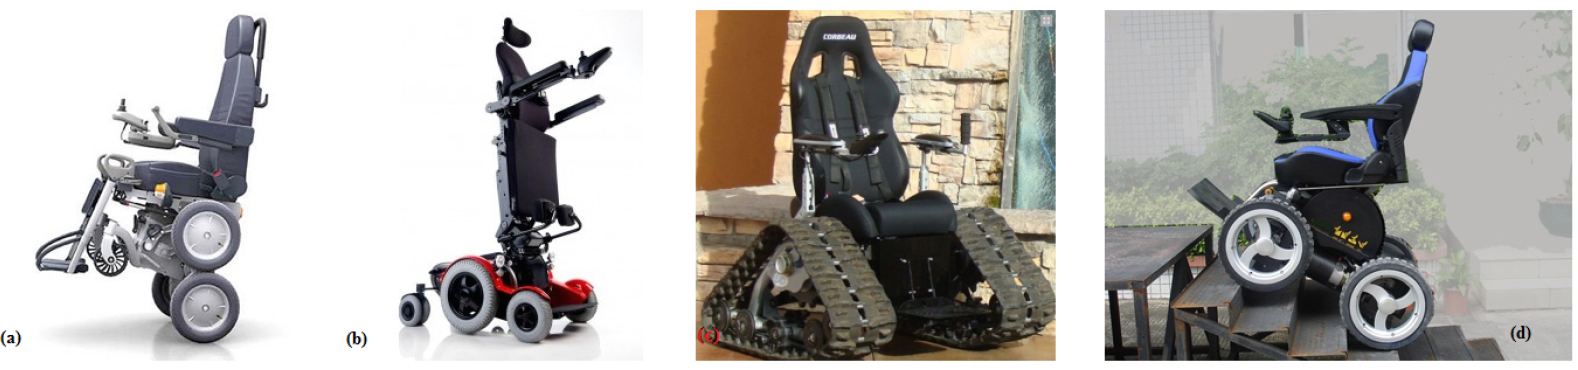
\includegraphics[width=1\textwidth]{fig/smart_wheel_chairs.png}
	\caption{近几年电动轮椅案例。}\label{fig:smart_wheel_chairs}
\end{figure*}
%%%%%%%%%%%%%%%%%

因此本文建模对象为电动轮椅中的机械与电驱动部分,如图\ref{fig:PW_rendering}所示。
首先,我们以两轮机器人系统理论应用与手动轮椅主体部分的分析,在此基础上,结合包括了电源,电机与驱动轮的便携式机电驱动模块(MDM, \textit{mechatronic drive modules}) 。该模块可以在必要时与大规模的手动轮椅系统耦合,以提高推进效率,从而给整体系统带来了很好的优势,因为模块的重量被施加在模块本身上,从而防止了结构的变形。考虑到复杂程度和所学知识,我们进行合理假设与简化模型,取整体系统的机械主体和附加机电模块,进行运动学仿真与键合图建模。

%%%%%%%%%%%%%%%%%
\begin{figure*}[!h]
	\centering
	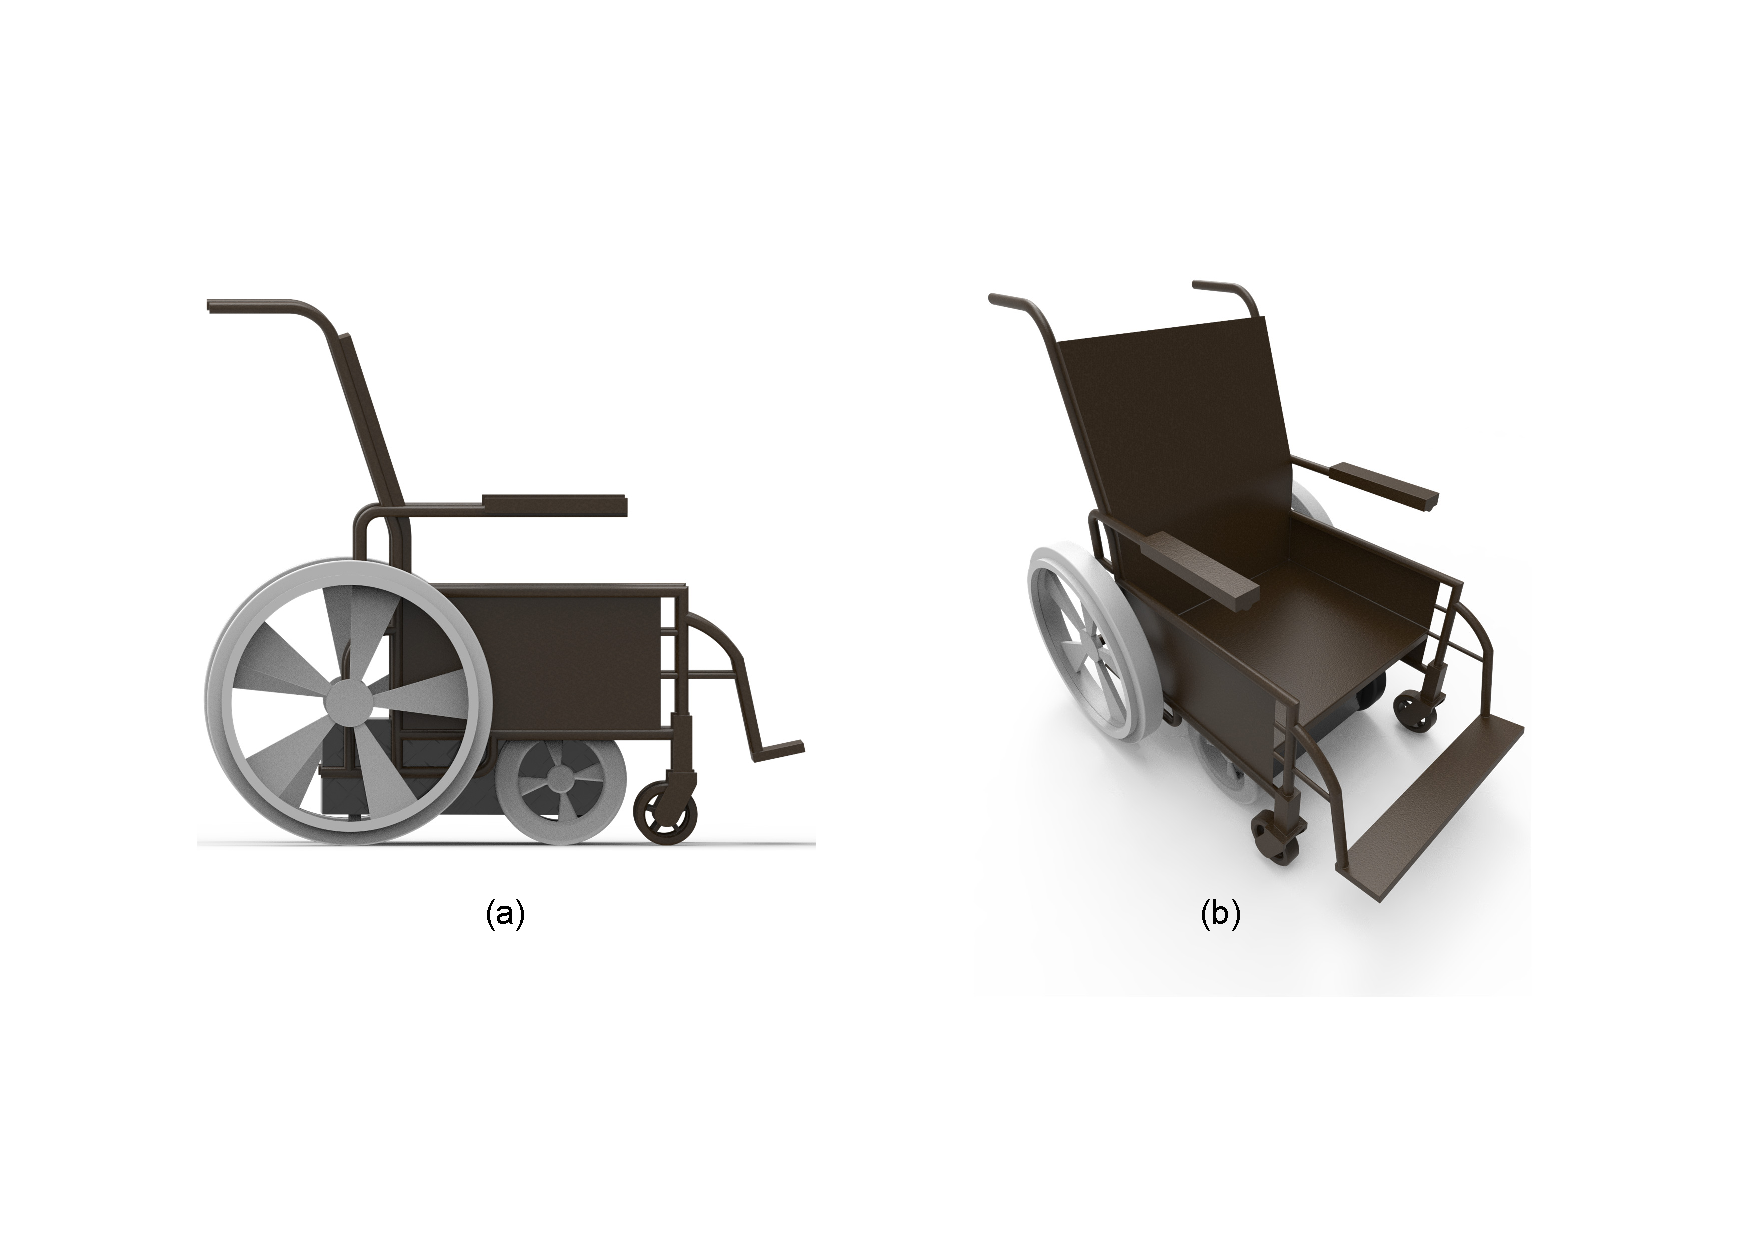
\includegraphics[width=1\textwidth]{fig/PW_rendering.pdf}
	\caption{选取电动轮椅示意。(a) 和 (b) 分别表示建模对象的侧视图和立体视图。}\label{fig:PW_rendering}
\end{figure*}
%%%%%%%%%%%%%%%%%

\subsection{本报告章节安排}

本报告从建模对象出发,从手推轮椅主体和机电驱动模块两部分出发进行分析建模,然后两部分结合进行系统整体分析总结,最后给出参考文献,报告主体内容包括以下几个部分:

第二章是对建模对象进行描述和问题提取,并给出相关模型合理假设以及参数标记;

第三章是对手推轮椅主体运动学分析和键合图建模;

第四章是对机电驱动模块的分析与键合图建模;

第五章是整体键合图的给出,并给出总结和分析;

最后部分为本文参考文献。
%\newpage
\section{任务介绍}

\subsection{建模对象描述}

所选定建模对象的系统特性将从\textbf{集合性、相关性、环境适应性}三个方面来分析。

\subsubsection{集合性}

该系统由机械主体模块和电驱动模块组成,二者缺一不可。 在创建物理设备建模仿真时,主要任务是实现集成控制驱动系统和执行器动态的模型,以便将仿真软件工具集成到模过程中。 

所谓执行机构在这里指的是机械主体模块,主要是由底盘与轮系。所谓控制驱动系统是指为机械系统提供动力的部分,这里主要指电驱动模块(如图~\ref{fig:PW_parts})。电驱动模块由电源,电机,齿轮等部分组成,电源供应整体电机及驱动的能量,电机转动先经过齿轮减速器减速增扭,最终传递到驱动轮轮系上,从而实现整体电动轮椅的功能。

\subsubsection{相关性}

就整体电动轮椅系统而言,子系统相互依存、相互制约、相互作用形成了相互关联的整体。

机械主体模块和电驱动模块间的联系是通过电机输出轴和驱动轮具有共同的位置和速度借助联轴器来实现的。通过电机轴的运动,实现驱动轮的转动。研究对象的机械主体和电驱动模块之间相互关联的变量是轴系转动的角速度。通过两者相互固定实现,势和流的传递。

%%%%%%%%%%%%%%%%%
\begin{figure*}[!h]
	\centering
	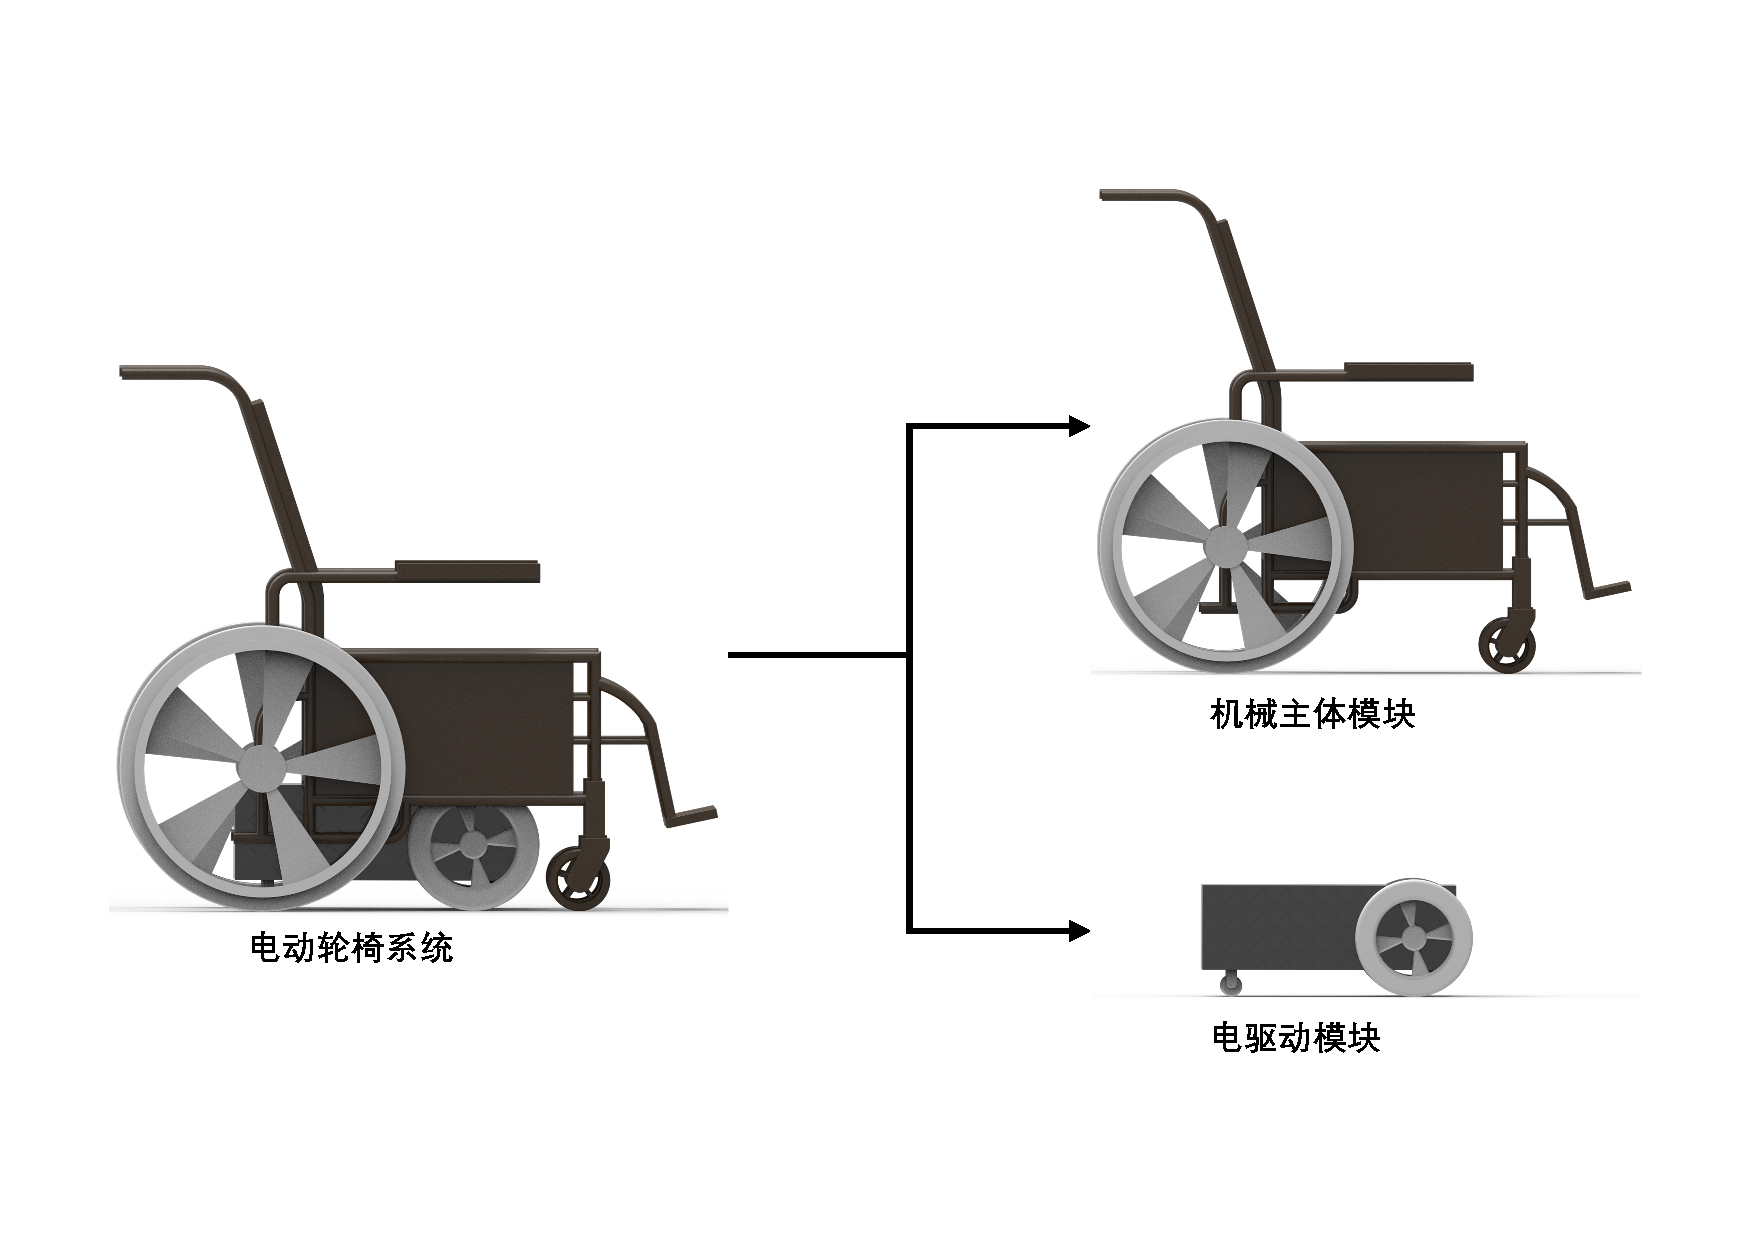
\includegraphics[width=0.95\textwidth]{fig/PW_parts.pdf}
	\caption{选取电动轮椅组成部分。}\label{fig:PW_parts}
\end{figure*}
%%%%%%%%%%%%%%%%%

\subsubsection{环境适应性}

传动的手推轮椅,结构简单,给行动不便人士以更大活动空间。但是在日常生活使用中,一般还是需要额外的人力用于前后左右前进与旋转运动。而机电模块的加入,将有效提高该设备的智能化程度,我们同时可以将相关移动机器人的控制分析理论应用其中。

在移动机器人中,主要分为轮式,履带式,足式等系统,通过机械与机电模块相结合,能够非常有效地处理平坦且结构良好的固体表面,从而满足行动不便人士的需求。

\subsection{建模问题提取}

可以将对象的工况分为两种情况:

\begin{enumerate}
	\item 在平坦路面上条件下,由人产生推力使轮椅向前运动。
	在该条件下,系统底部受到的速度输入较小且较不稳定。主要考虑以下几个参数:
	\begin{itemize}
		\item 车轮转动惯量,转动惯量;
		
		\item 车轮辐条刚度:存在于从车轮中心到地面由于充气轮胎所带来的弹簧/阻尼;
		
		\item 摩擦损失:存在于后充气轮和前脚轮与地面之间的阻力;
		
		\item 质量:包括椅子的重量和使用者的假定质量。该点位于重心处,获得系统平均质量。在降低模型的复杂性时,假设重心与后轮轴线中心重合。
	\end{itemize}
	
	\item 在平坦路面上条件下,由机电驱动模块产生使轮椅向前运动的动力。
	在该条件下,系统底部受到的速度输入较大且较稳定。主要考虑以下几个参数:
	\begin{itemize}
		\item 直流电动机的基本原理(包括电感,输出扭矩等)和基本性质(包括质量,电压等)。
		
		\item 传动部件的刚度,质量以及机械损失。
		
		\item 电动轮的转动惯量。
	\end{itemize}
	
\end{enumerate}

\subsection{模型假设与标记}

\subsubsection{模型假设}

针对上述工况,结合简化模型的角度出发,做出如下假设:

\begin{itemize}
	
	\item 假设机械各部分零件为刚体;
	
	\item 假设刚体质心位于几何中心;
	
	\item 忽略铰接点连接处的摩擦;
	
	\item 忽略电驱动系统工作产热带来的参数变化。
	
\end{itemize}

\subsubsection{参数及其数学标记}

表 \ref{tab:param} 列出本模型的相关参数及其数学标记。本报告中表示左右参数则分别以 $ \_L $ 和 $ \_R $表示。参数表主要分为分为整体系统参数,手推轮椅主体,机电驱动模块以及手推控制输入部分的参数四个部分。如下所示(见下页):

\begin{table}[H]
\footnotesize
\caption{系统主要参数及其数学标记}\label{tab:param}
\begin{longtable}{l|l}
	\toprule
	\textbf{数学标记} & \textbf{系统参数}\\
	\midrule
	\endhead
	\multicolumn{2}{l}{\textbf{系统整体参数}} \\ % {占用行数} {文字居左中右} {内容}
	\midrule
	$ M $ & 总体质量\\
	$ J $ & 总体转动惯量\\
	$ V_{\rm{CG}} $ & 质心速度\\
	$ w_{\rm{CG}} $ & 质心转速\\
	$ P_{\rm{CG}} $ & 系统动量变化率\\
	$ P_{\theta} $ & 系统角动量变化率\\
	\midrule
	\multicolumn{2}{l}{\textbf{手推轮椅主体}} \\
	\midrule
	SE:$\tau$ & 后轮推进扭矩 \\
	$ J w $ & 后轮转动惯量\\
	$ M_t $ & 系统质量\\
	$ J t $ & 系统转动惯量\\
	$ R_g $ & 轮胎与地面摩擦系数\\
	$ C_w $ & 轮辐弹性系数\\
	$ R_w $ & 轮辐阻尼\\
	$ r $ & 后轮半径\\
	$ L_w $ & 轮椅宽度\\
	$ R_{wC} $ & 联轴器系数\\
	\midrule
	\multicolumn{2}{l}{\textbf{机电驱动模块}} \\
	\midrule
	$ I_e $ & 电机电感\\
	$ R_e $ & 电机内阻\\
	$ J_r $ & 转子转动惯量\\
	$ R_b $ & 电机轴承阻尼\\
	$ M_d $ & 机电驱动模块质量\\
	$ J_d $ & 机电驱动模块转动惯量\\
	$ L_d $ & 模块宽度\\
	$ C_s $ & 电机输出转矩\\
	$ R_s $ & 电机输出轴阻尼\\
	$ k_1 $ & 电机扭矩系数\\ % 简化了k8
	$ k_2 $ & 齿轮系数比\\ % 简化了k7
	$ k_3 $ & 电动车轮半径 \\ % 简化了k6
	Se:L & 输入控制电压\\
	\midrule
	\multicolumn{2}{l}{\textbf{手推控制输入部分}}\\
	\midrule
	$ J $ & 手动轮转动惯量\\
	$ k_4 $ & 手动轮半径\\ % 简化了k10
	\bottomrule
\end{longtable}
\end{table}
%\input{data/3.Electrical}
%\clearpage
\section{系统总体模型}

在本文中,在将原有的机械主体部分和电驱动模块连接在一起,我们便得到了总体的键合图,从而验证最初的系统分析的合理性,机械主题部分和电驱动模块的
通过机械连接后,便生成了总体键合图,如下图~\ref{fig:overall}所示。

%%%%%%%%%%%%%%%%%
\begin{figure*}[!h]
	\centering
	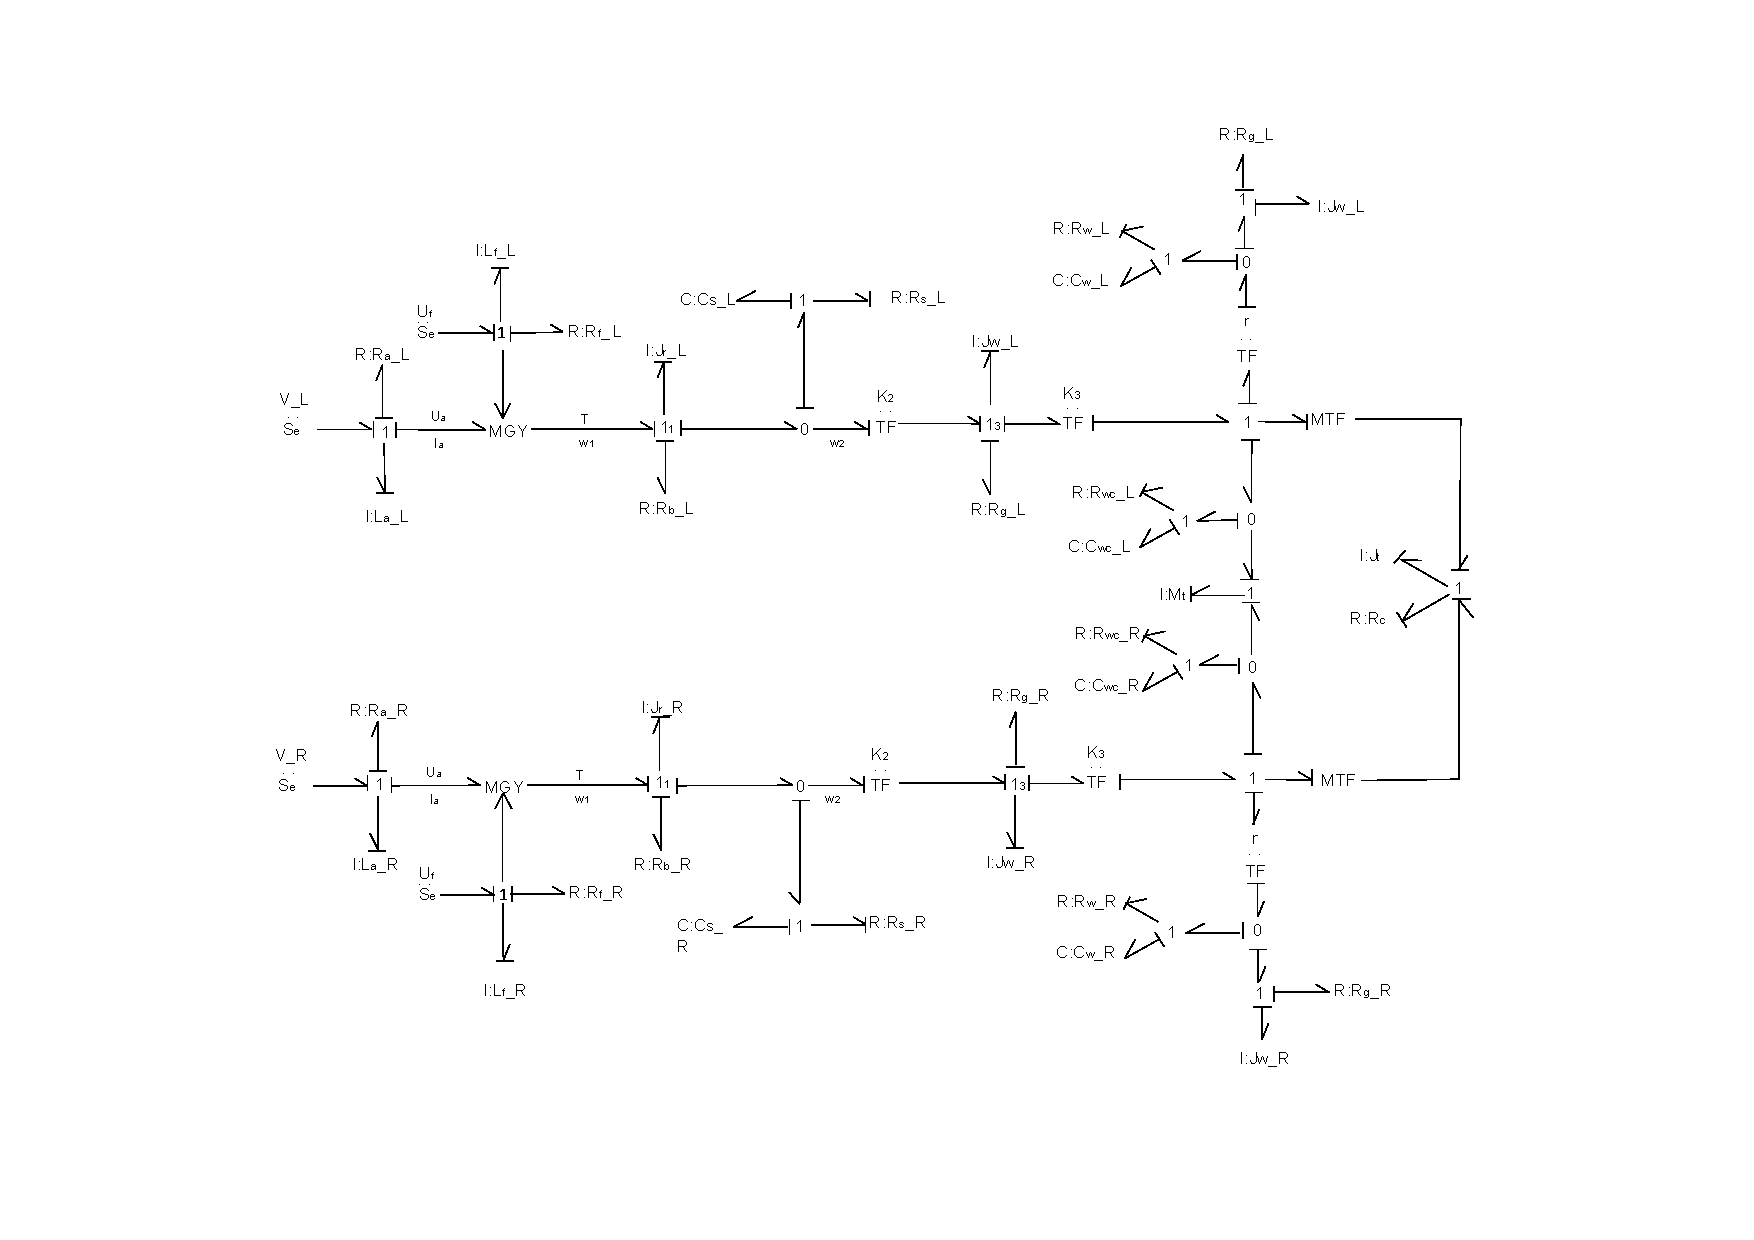
\includegraphics[width=1.25\textwidth,angle=90]{fig/overall.pdf}
	\caption{总体键合图。}\label{fig:overall}
\end{figure*}
%%%%%%%%%%%%%%%%%
%\newpage
\addcontentsline{toc}{section}{参考文献}
\begin{thebibliography}{0}
	
	\bibitem{System_Dynamics_Modeling}
	D. C. Karnopp, D. L. Margolis, and R. C. Rosenberg, System Dynamics Modeling and Simulation of Mechatronic Systems (Fourth Edition) [M]. New York: Wiley, 2012.
		
	\bibitem{System_Dynamics_Modeling_cn}
	D. C. Karnopp, D. L. Margolis, and R. C. Rosenberg, 黎明安(译), 系统动力学——机电系统的建模与仿真 [M]. 国防工业出版社, 2012.
	
	\bibitem{Simulation1}
	Klee H , Allen R . Simulation of dynamic systems with MATLAB and Simulink. 2nd ed[M]// Simulation of Dynamic Systems with MATLAB and Simulink. CRC Press, Inc. 2007.
	
	\bibitem{Simulation2}
	Wouwer A V . Simulation Of ODE/PDE Models With MATLAB®, OCTAVE And SCILAB[J]. Annals of the Rheumatic Diseases, 2014, 71(Suppl 3):646-646.
	
	\bibitem{wheelchairs_review}
	Leaman, Jesse, and Hung Manh La. A comprehensive review of smart wheelchairs: past, present, and future [J]. IEEE Transactions on Human-Machine Systems 47.4 2017: 486-499.
	
	\bibitem{Bond_graph_methodology}
	Borutzky, W. Bond graph methodology, development and analysis of multidisciplinary dynamic system models (1st ed.) [M]. Berlin: Springer. 2010
	
	\bibitem{Bond_graph_modelling}
	Borutzky, Wolfgang. Bond graph modelling of engineering systems  [M]. Vol. 103. New York: Springer, 2011.
	
	\bibitem{Ayala2015ROBIO}
	Ayala, Gerardo, Rui Loureiro, and Rochdi Merzouki. Multi-domain model of steering system for an omnidirectional mobile robot  [C]. 2015 IEEE International Conference on Robotics and Biomimetics (ROBIO). IEEE, 2015.
	
	\bibitem{Sahoo2016RCTFC}
	Sahoo, Saumya Ranjan, and Shital S. Chiddarwar. Dynamic modelling of four wheel skid mobile robot by unified bond graph approach [C]. 2016 International Conference on Robotics: Current Trends and Future Challenges (RCTFC). IEEE, 2016.
	
	\bibitem{Jahanbin2016JBSMSE}
	Jahanbin, Zahra, et al. Multi-body simulation of a flapping-wing robot using an efficient dynamical model [J]. Journal of the Brazilian Society of Mechanical Sciences and Engineering 38.1 (2016): 133-149.
	
	\bibitem{Proceedings1}
	Fakri, A., Vilakazi, J. P. Modular driven wheelchair bond graph modelling [C]. The European Modeling \& Simulation Symposium, I3M2010 MultiConference, 2010, Fes, Morocco.
	
	\bibitem{Proceedings2}
	Fakri, A., Vilakazi, J. P. Wheelchair and electric drive add-on a whole bond graph modelling [C]. Proceedings of the 2014 11th International Conference on Bond graph Modeling and Simulation (ICBGM’14). SummerSim 2014 Multiconference July 6–10 2014, Monterey, CA, USA. ISBN: 978-1-63266-700-7, Vol. 46 \#8, Collection:Simulation Series, 206-210, 222 pp. 113.
	
\end{thebibliography}
%\newpage
\section{绪论}

%——————————————————————图片格式——————————————————————	
\begin{figure}[htbp]
	\centering
	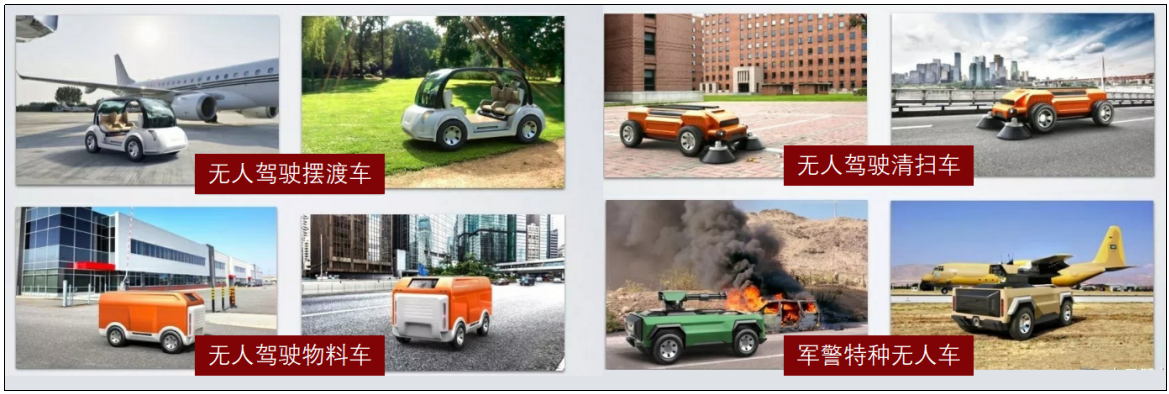
\includegraphics[width = 1\textwidth]{fig/wlknyy.png}
	\caption{未来可能应用}
	\label{wlknyy}
\end{figure}

%——————————————————————表格格式——————————————————————	
\begin{table}[htbp]
	\centering%表格居中
	\caption[centering]{The average daily use of sharing bicycles \protect\\and the number of bikes at the same period}%表格标题
	\label{共享单车日均使用总量与对应时间段的共享单车数量}%表格标签
	\begin{tabular}{ccc}
%	\begin{tabular}{C{4cm}C{4cm}C{3.5cm}}	
		\toprule
		\tabincell{c}{Averagedaily use\\(per 10000 people)} &\tabincell{c}{Sharing bicycles\\(per 10000 bikes)} &\tabincell{c}{Period}\\ 
		\midrule
		402.4 & 95 & 10.31$\sim$11.06 \\
		418.7 & 99 & 11.07$\sim$11.13 \\
		477.8 & 102 & 11.14$\sim$11.20 \\
		440.7 & 106 & 11.21$\sim$11.27 \\
		589.7 & 110 & 11.28$\sim$12.04 \\
		636.8 & 114 & 12.05$\sim$12.11 \\
		716.8 & 117 & 12.12$\sim$12.18 \\
		716.6 & 121 & 12.19$\sim$12.25 \\
		728.6 & 125 & 12.26$\sim$01.01 \\
		738.6 & 129 & 01.02$\sim$01.08 \\
		747.2 & 132 & 01.09$\sim$01.15 \\
		946.4 & 147 & 02.06$\sim$02.12 \\
		1047.1 & 151 & 02.13$\sim$02.19 \\
		1173.6 & 155 & 02.20$\sim$02.26 \\
		\bottomrule
	\end{tabular}
\end{table}

%——————————————————————对齐样式——————————————————————

一行对齐:\leftline{左对齐} \centerline{居中} \rightline{右对齐}
多行或者段落对齐:
左对齐 \begin{flushleft}...\end{flushleft}
居中 \begin{center}...\end{center}
右对齐 \begin{flushright}...\end{flushright}

%——————————————————————参考文献样式——————————————————————

%\section*{参考资料}
\addcontentsline{toc}{section}{参考文献}
\begin{thebibliography}{0}
		\bibitem{sj}
		赵瑜, 闫宏伟. 履带式行走机构设计分析和研究[J]. 新技术新工艺, 2010(5):50-53.
		
		\bibitem{dpsj}
		诸文农. 底盘设计[M]. 机械工业出版社, 2001.
	
\end{thebibliography}


\end{document}
